\documentclass[10pt]{article}

\usepackage{geometry}
\geometry{margin = 3em,top =6em, headheight=\paperheight}
\usepackage[export]{adjustbox}
\usepackage{array}
\usepackage{amsmath}
\usepackage{amsfonts}
\usepackage{fancyhdr}
\pagestyle{fancy}
\fancyhf{}
\lhead{Algebra II}
\chead{Function  Characteristics}
\rhead{Action Opportunity B, Page \thepage}
\usepackage{lastpage}
\usepackage{xcolor}
\usepackage{enumitem}
\usepackage{pifont}
\usepackage{graphicx}
\graphicspath{{../img}}
\usepackage{pgfplots}
\pgfplotsset{compat=1.18}
\usepackage{tabularx}

\newcommand{\R}{\mathbb R}
\newcommand{\e}{{\rm e}}
\newcommand{\pobr}[1]{\left\langle#1\right\rangle}
\newcommand{\norm}[1]{\lVert #1 \rVert}
\newcommand{\abs}[1]{\lvert #1 \rvert}

\DeclareMathOperator{\xd}{d\!}
\DeclareMathOperator{\proj}{proj}

\title{}
\date{}

\begin{document}
\noindent
{\large
Name \rule{16em}{.5pt}\hspace{\stretch{1}} Date \rule{8em}{.5pt}\hspace{\stretch{1}} Period \rule{2em}{.5pt}
}
\vspace{1em}

\begingroup
\renewcommand{\arraystretch}{1.5}
\begin{center}
{\footnotesize
\begin{tabularx}{\textwidth}{|X|X|X|X|X|X|}
\hline
\bf BE PRECISE & \centerline{Integrating} & \centerline{Applying} & \centerline{Practicing} & \centerline{Acquiring} & \centerline{Awaiting Evidence} \\
\hline
I can calculate accurately and efficiently, and be precise in all of my math.&
Selects and applies the correct procedure and solves all routine AND integrating problems.

AND

Expresses the answer to the correct level of precision needed for the problem (including the correct rounding, units, math symbols, labeling, graphing, vocab…)
&Selects and applies the correct procedure and solves all routine problems.


AND

Expresses the answer to the correct level of precision needed for the problem (including the correct rounding, units, math symbols, labeling, graphing, vocab…)
&Selects and applies the correct procedure and solves most routine problems.


AND

Expresses the answer to the correct level of precision needed for the problem (including the correct rounding, units, math symbols, labeling, graphing, vocab…)
&Selects and applies the correct procedure and solves some routine problems.


AND

Attempts to express the answer to the correct level of precision needed for the problem (including the correct rounding, units, math symbols, labeling, graphing, vocab…).
&Selects and attempts to apply the correct procedure for some routine problems.\\
\hline
\bf Criteria&\multicolumn{5}{l|}{\parbox[c][4em]{.8\textwidth}{When describing the graph, you have to address, if exists, the $x$-intercept, $y$-intercept, maxima and minima (both absolute and relative), asymptotes, symmetric axes, and the period.}}\\
\hline
\end{tabularx}
}
\end{center}
\endgroup
\vspace{2em}

\begin{enumerate}
\item Describe the following graph.

\begin{center}
\begin{tabular}{p{0.5\textwidth}p{0.5\textwidth}}
\parbox{0.5\textwidth}{
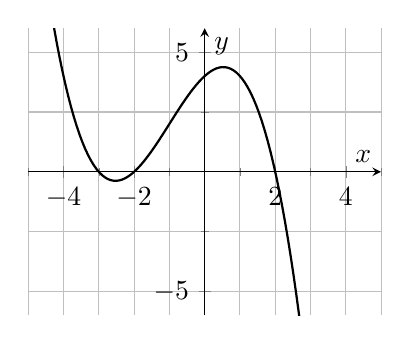
\begin{tikzpicture}
\begin{axis}[
    xlabel={$x$},
    ylabel={$y$},
    grid=both,
    minor tick num=1,
    axis lines=middle,
    xmin=-5,xmax=5,
    ymin=-6,ymax=6,
    domain=-5:3,
    samples=100,
    width=0.5\textwidth
]
\addplot[thick]{-(x+3)*(x+2)*(x-2)/3};
\end{axis}
\end{tikzpicture}
}&\parbox[c]{0.5\textwidth}{{\bf \large Description}\\[1.5em]
\rule{0.4\textwidth}{0.5pt}\\[1.5em]
\rule{0.4\textwidth}{0.5pt}\\[1.5em]
\rule{0.4\textwidth}{0.5pt}\\[1.5em]
\rule{0.4\textwidth}{0.5pt}\\[1.5em]
\rule{0.4\textwidth}{0.5pt}\\[1.5em]
\rule{0.4\textwidth}{0.5pt}\\[1.5em]
\rule{0.4\textwidth}{0.5pt}\\[1.5em]
}
\end{tabular}
\end{center}
\item Let \(f(x) = x^2 + 5x + 4\).  Find the zeros, the $y$-intercept and the vertex of the graph of $f(x)$, then plot the graph.
\end{enumerate}
\end{document}